\documentclass[class=jsarticle, crop=false, dvipdfmx, fleqn]{standalone}
%% preamble for Numerical-structure-analysis report

\input{/Users/User/Documents/Project/TeX/preamble/mypreamble}

%% titles
\title{統計的機械学習 レポート}
\author{37-196360 \quad 森田涼介}


%% setting for listings
\newtcbinputlisting[auto counter]{\reportlisting}[3][]{%
	listing file = {#3},
	listing options = {language=python, style=tcblatex, numbers=left, numberstyle=\tiny},
	listing only,
	breakable,
	toprule at break = 0mm,
	bottomrule at break = 0mm,
	left = 6mm,
	sharp corners,
	drop shadow,
	title = Listings \thetcbcounter : \texttt{#2},
	label = #1,
	}



%% title format
\usepackage{titlesec}
\titleformat{\section}{\LARGE}{宿題\thesection}{0zw}{}
\newcommand{\sectionbreak}{\clearpage}
\titleformat{\subsection}{\Large}{\Alph{subsection})}{0zw}{}

\begin{document}
\section{}

射影追跡の近似ニュートンアルゴリズムを実装する。


\subsection*{理論}

i.i.dな標本\(\qty{\bm{x}_i}_{i=1}^{n},\ (\bm{x}_i \in \mathbb{R}^d)\)に対して射影追跡を行うことを考える。
標本を中心化・球状化したものを\(\qty{\tilde{\bm{x}}_i}_{i=1}^{n}\)とし,
以降はこれについて考える。
\(\bm{b}\ (\in \mathbb{R}^d)\)によって射影するとすれば,
射影方向\(\bm{b}\)の非ガウス性は
\begin{equation}
    s = \Braket{\bm{b},\ \tilde{\bm{x}}} \qquad (||\bm{b}|| = 1)
\end{equation}
によって測ることができる。
また,非ガウス性尺度を\(G(s)\)の期待値\(E\qty[G(s)]\)とする。
これを最大化するような\(\bm{b}\)が求まればよい。
なお,\(G(s)\)としては様々な関数が考えられるが,
例えば\(G(s) = s^4\)とすれば,これは尖度を表す。

いま,標本を用いて\(G(s)\)の期待値を表すと,
\begin{align}
    & E\qty[G(s)] = \frac{1}{n} \sum_{i=1}^{n} G(s_i) \\
    & s_i = \Braket{\bm{b},\ \tilde{\bm{x}}_i}, \quad ||\bm{b}|| = 1
\end{align}
となる。
これをラグランジュの未定乗数法で最大化することを考える。
\begin{equation}
    L\qty[\bm{b},\ \lambda] = \frac{1}{n} \sum_{i=1}^{n} G(s_i) + \lambda (||\bm{b}|| - 1)
\end{equation}
\(\pdv*{s_i}{\bm{b}} = \tilde{\bm{x}}_i\)に注意すると,
ラグランジアンの\(\bm{b}\)による偏微分は,
\begin{equation}
    \pdv{L}{\bm{b}} = \frac{1}{n} \sum_{i=1}^{n} \tilde{\bm{x}}_i G^\prime (s_i) + 2 \lambda\bm{b}
\end{equation}
近似ニュートン法により,\(\pdv*{L}{\bm{b}} = \bm{0}\)となるような\(\bm{b}\)を探す。
\begin{equation}
    f(\bm{b}) = \pdv{L}{\bm{b}} = \frac{1}{n} \sum_{i=1}^{n} \tilde{\bm{x}}_i G^\prime (s_i) + 2 \lambda\bm{b}
\end{equation}
とおくと,
\(\bm{b}\)の更新式は次で与えられる。
\begin{equation}
    \bm{b} \leftarrow \bm{b} - \qty(\pdv{f}{\bm{b}})^{-1} f(\bm{b})
\end{equation}
ここで,
\begin{equation}
    \pdv{f}{\bm{b}}
        = \pdv[2]{L}{\bm{b}}{\bm{b}^\mathrm{T}}
        = \frac{1}{n} \sum_{i=1}^{n} \tilde{\bm{x}}_i \tilde{\bm{x}}_i^\mathrm{T} G^{\prime\prime} (s_i) + 2 \lambda\bm{I}_d
\end{equation}
であり,
\begin{equation}
    \frac{1}{n} \sum_{i=1}^{n} \tilde{\bm{x}}_i \tilde{\bm{x}}_i^\mathrm{T} G^{\prime\prime} (s_i)
        \sim \frac{1}{n} \sum_{i=1}^{n} G^{\prime\prime} (s_i) \bm{I}_d
\end{equation}
と近似すると,結局
\begin{align}
    \pdv{f}{\bm{b}}
        & \sim \frac{1}{n} \sum_{i=1}^{n} G^{\prime\prime} (s_i) \bm{I}_d + 2\lambda\bm{I}_d \\
        & = \qty(\frac{1}{n} \sum_{i=1}^{n} G^{\prime\prime} (s_i) + 2\lambda) \bm{I}_d \\
\end{align}
となり,これより,
\begin{equation}
    \qty(\pdv{f}{\bm{b}})^{-1} = \frac{1}{\frac{1}{n} \sum_{i=1}^{n} G^{\prime\prime} (s_i) + 2\lambda} \bm{I}_d
\end{equation}
を得る。
以上より,\(\bm{b}\)の更新式は次のようになる。
\begin{align}
    \bm{b}
        & \leftarrow \bm{b} - \qty(\pdv{f}{\bm{b}})^{-1} f(\bm{b}) \\
        & = \bm{b} - \frac{1}{\frac{1}{n} \sum_{i=1}^{n} G^{\prime\prime} (s_i) + 2\lambda} \bm{I}_d \qty(\frac{1}{n} \sum_{i=1}^{n} \tilde{\bm{x}}_i G^\prime (s_i) + 2 \lambda\bm{b}) \\
        & = \frac{1}{\frac{1}{n} \sum_{i=1}^{n} G^{\prime\prime} (s_i) + 2\lambda} \qty{\qty(\frac{1}{n} \sum_{i=1}^{n} G^{\prime\prime} (s_i)) \bm{b} - \frac{1}{n} \sum_{i=1}^{n} \tilde{\bm{x}}_i G^\prime (s_i)}
\end{align}
\(\bm{b}\)は更新の後正規化されるため,結局,
\begin{equation}
    \bm{b} \leftarrow \qty(\frac{1}{n} \sum_{i=1}^{n} G^{\prime\prime} (s_i)) \bm{b} - \frac{1}{n} \sum_{i=1}^{n} \tilde{\bm{x}}_i G^\prime (s_i)
\end{equation}
とすればよい。



\subsection*{問題設定}

非ガウス性尺度を,次の3つの関数とした場合について考える。
\begin{align}
    & G(s) = s^4 \\
    & G(s) = \log(\cosh(s)) \\
    & G(s) = - \exp(- \frac{s^2}{2})
\end{align}
サンプルは,\(x\)軸を一様分布,\(y\)軸を標準正規分布からサンプリングしたのち,
適当な変換をかけて白色化したものとする。
また,これは1点だけ外れ値を含む。
サンプル数は\(n = 1,000,\ 1,500,\ 10,000\)の3段階について考えた。

また,収束の条件は,
現在の\(\bm{b}\)直近5イタレーションにおける\(\bm{b}\)のそれぞれについてEuclid距離を計算し,
そのうちの最大値が\num{1e-4}以下になったときとした。

なお,プログラムは\pageref{listing:assignment2}ページのListing \ref{listing:assignment2}に示した。



\subsection*{結果}

各設定について,\(\bm{b}\)の描かれた散布図,
及びそこにサンプルを射影したときのヒストグラムを示す。
図\ref{fig:s4_n1000}--\ref{fig:s4_n10000}に\(G(s) = s^4\),
図\ref{fig:logcosh_n1000}--\ref{fig:logcosh_n10000}に\(G(s) = s^4\),
図\ref{fig:exp_n1000}--\ref{fig:exp_n10000}に\(G(s) = s^4\)
の結果を示した。

結果を見ると,サンプル数1,000ではどのモデルも外れ値に引っ張られてしまい,
いい射影を得られていないことがわかる。
また,サンプル数を10,000まで増やせば,どのモデルでも外れ値の影響はなくなっている。
違いが出ているのはサンプル数1,500のときで,
このとき,\(G(s) = s^4\)のモデルのみ外れ値の影響を大きく受けてしまっている。
このことから,非ガウス性を評価する際に外れ値の存在が予想される場合は,
尖度以外の指標を用いた方がよりよい射影を得られる可能性が高そうであるということが分かった。


\clearpage
\begin{figure}
	\centering
    \begin{minipage}{0.45\linewidth}
        \begin{figure}[H]
        	   \centering
            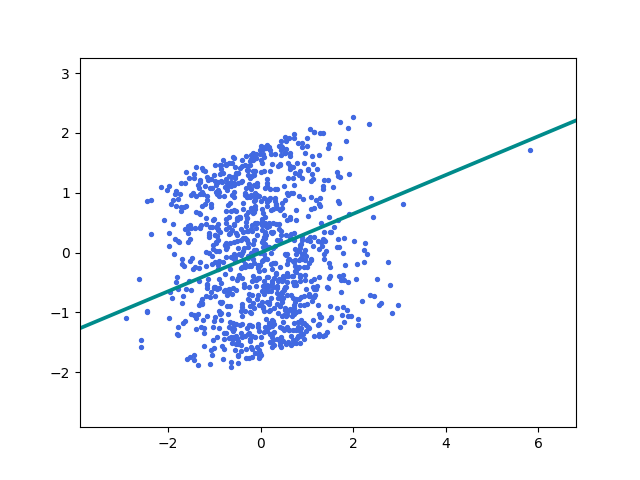
\includegraphics[clip, width=\linewidth]{../figures/assignment2_result_s4_n1000_scatter.png}
            \subcaption{散布図}
            \label{fig:s4_n1000_scatter}
        \end{figure}
    \end{minipage}
    \begin{minipage}{0.45\linewidth}
        \begin{figure}[H]
            \centering
            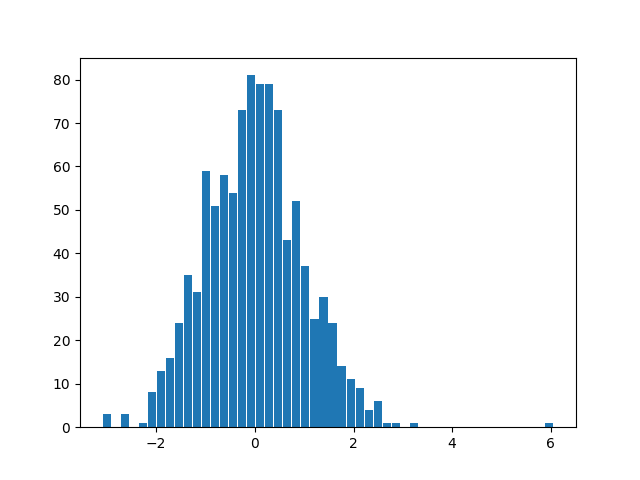
\includegraphics[clip, width=\linewidth]{../figures/assignment2_result_s4_n1000_hist.png}
            \subcaption{ヒストグラム}
            \label{fig:s4_n1000_hist}
        \end{figure}
    \end{minipage}
    \caption{非ガウス性尺度\(G(s) = s^4\),標本数1,000のときの散布図と射影方向,及びヒストグラム}
    \label{fig:s4_n1000}
\end{figure}

\begin{figure}
	\centering
    \begin{minipage}{0.45\linewidth}
        \begin{figure}[H]
        	   \centering
            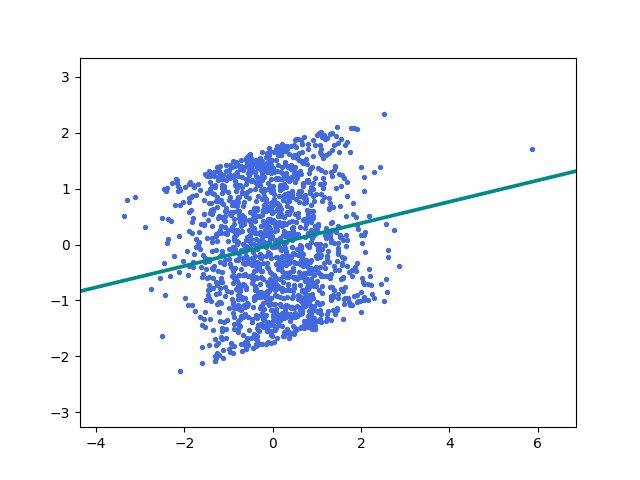
\includegraphics[clip, width=\linewidth]{../figures/assignment2_result_s4_n1500_scatter.png}
            \subcaption{散布図}
            \label{fig:s4_n1500_scatter}
        \end{figure}
    \end{minipage}
    \begin{minipage}{0.45\linewidth}
        \begin{figure}[H]
            \centering
            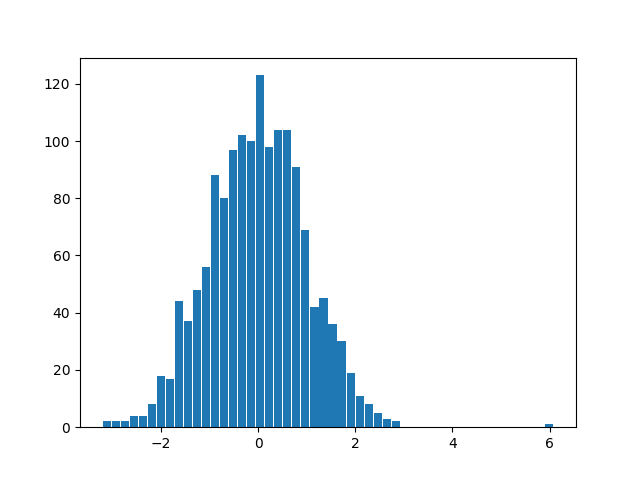
\includegraphics[clip, width=\linewidth]{../figures/assignment2_result_s4_n1500_hist.png}
            \subcaption{ヒストグラム}
            \label{fig:s4_n1500_hist}
        \end{figure}
    \end{minipage}
    \caption{非ガウス性尺度\(G(s) = s^4\),標本数1,500のときの散布図と射影方向,及びヒストグラム}
    \label{fig:s4_n1500}
\end{figure}

\begin{figure}
	\centering
    \begin{minipage}{0.45\linewidth}
        \begin{figure}[H]
        	   \centering
            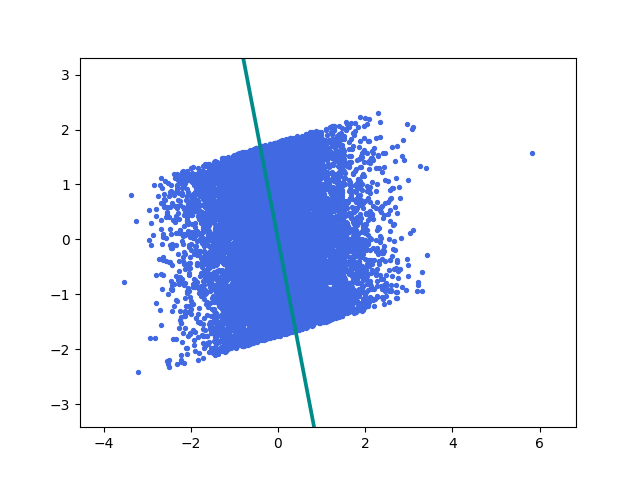
\includegraphics[clip, width=\linewidth]{../figures/assignment2_result_s4_n10000_scatter.png}
            \subcaption{散布図}
            \label{fig:s4_n10000_scatter}
        \end{figure}
    \end{minipage}
    \begin{minipage}{0.45\linewidth}
        \begin{figure}[H]
            \centering
            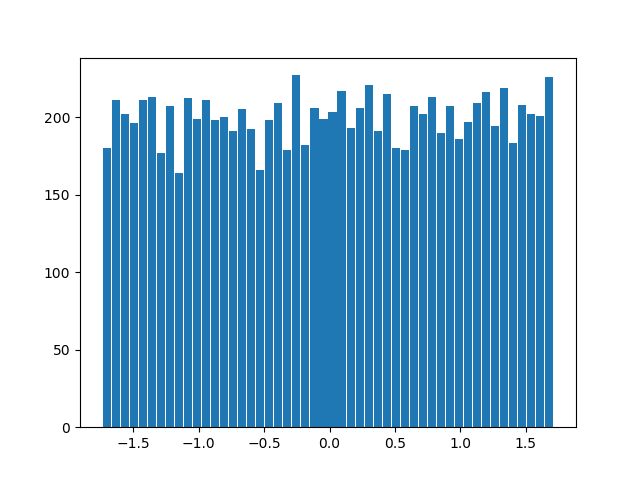
\includegraphics[clip, width=\linewidth]{../figures/assignment2_result_s4_n10000_hist.png}
            \subcaption{ヒストグラム}
            \label{fig:s4_n10000_hist}
        \end{figure}
    \end{minipage}
    \caption{非ガウス性尺度\(G(s) = s^4\),標本数10,000のときの散布図と射影方向,及びヒストグラム}
    \label{fig:s4_n10000}
\end{figure}


\clearpage
\begin{figure}
	\centering
    \begin{minipage}{0.45\linewidth}
        \begin{figure}[H]
        	   \centering
            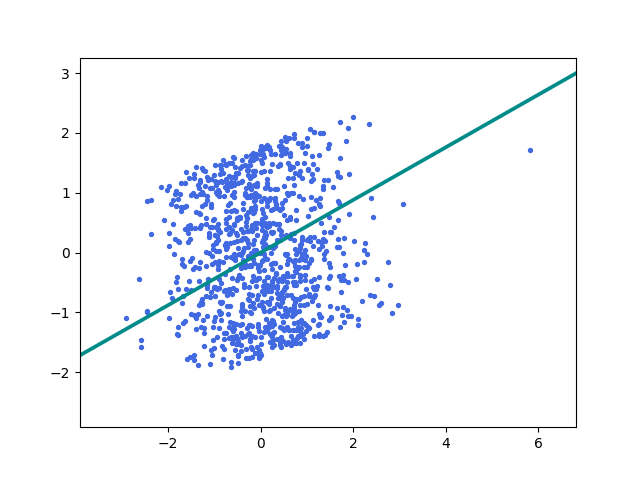
\includegraphics[clip, width=\linewidth]{../figures/assignment2_result_logcosh_n1000_scatter.png}
            \subcaption{散布図}
            \label{fig:logcosh_n1000_scatter}
        \end{figure}
    \end{minipage}
    \begin{minipage}{0.45\linewidth}
        \begin{figure}[H]
            \centering
            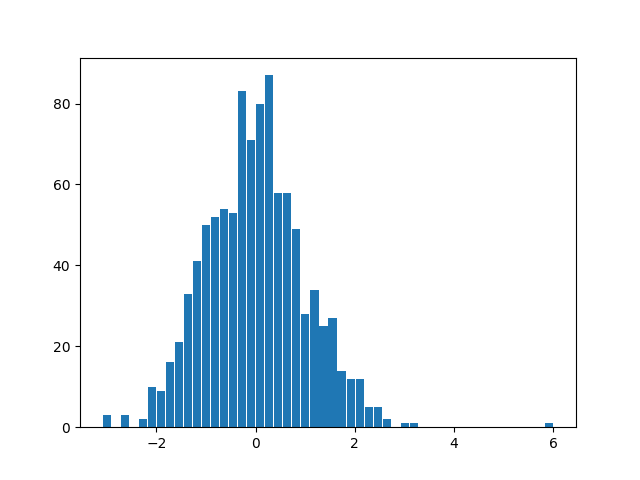
\includegraphics[clip, width=\linewidth]{../figures/assignment2_result_logcosh_n1000_hist.png}
            \subcaption{ヒストグラム}
            \label{fig:logcosh_n1000_hist}
        \end{figure}
    \end{minipage}
    \caption{非ガウス性尺度\(G(s) = \log\cosh(s)\),標本数1,000のときの散布図と射影方向,及びヒストグラム}
    \label{fig:logcosh_n1000}
\end{figure}

\begin{figure}
	\centering
    \begin{minipage}{0.45\linewidth}
        \begin{figure}[H]
        	   \centering
            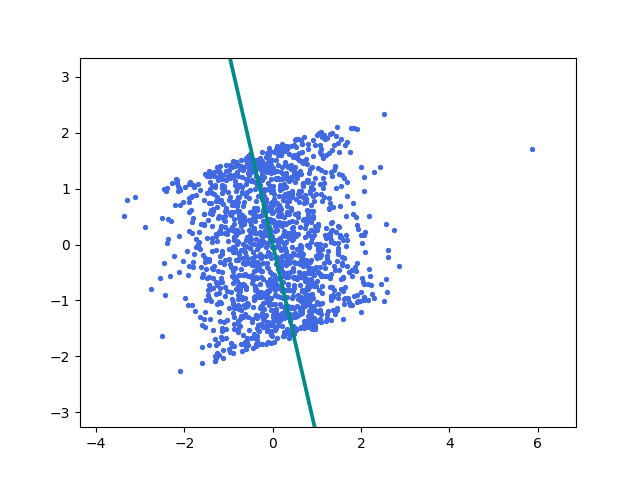
\includegraphics[clip, width=\linewidth]{../figures/assignment2_result_logcosh_n1500_scatter.png}
            \subcaption{散布図}
            \label{fig:logcosh_n1500_scatter}
        \end{figure}
    \end{minipage}
    \begin{minipage}{0.45\linewidth}
        \begin{figure}[H]
            \centering
            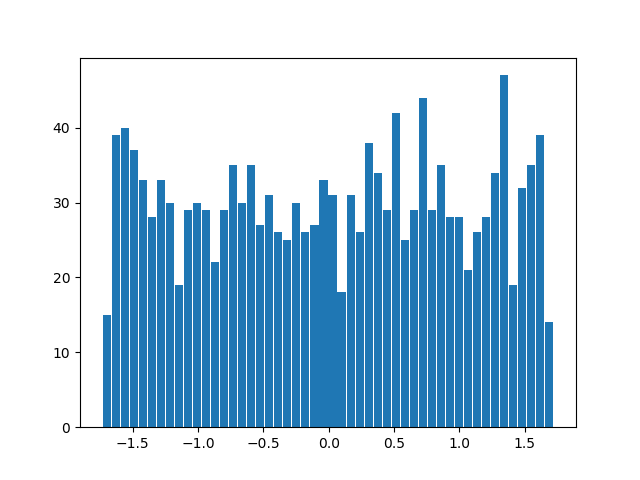
\includegraphics[clip, width=\linewidth]{../figures/assignment2_result_logcosh_n1500_hist.png}
            \subcaption{ヒストグラム}
            \label{fig:logcosh_n1500_hist}
        \end{figure}
    \end{minipage}
    \caption{非ガウス性尺度\(G(s) = \log\cosh(s)\),標本数1,500のときの散布図と射影方向,及びヒストグラム}
    \label{fig:logcosh_n1500}
\end{figure}

\begin{figure}
	\centering
    \begin{minipage}{0.45\linewidth}
        \begin{figure}[H]
        	   \centering
            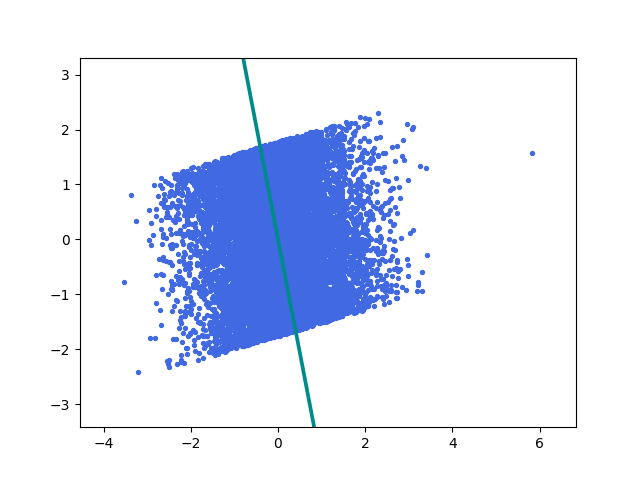
\includegraphics[clip, width=\linewidth]{../figures/assignment2_result_logcosh_n10000_scatter.png}
            \subcaption{散布図}
            \label{fig:logcosh_n10000_scatter}
        \end{figure}
    \end{minipage}
    \begin{minipage}{0.45\linewidth}
        \begin{figure}[H]
            \centering
            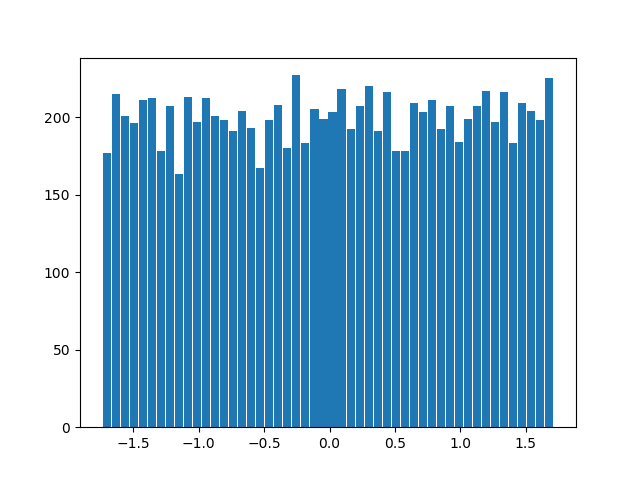
\includegraphics[clip, width=\linewidth]{../figures/assignment2_result_logcosh_n10000_hist.png}
            \subcaption{ヒストグラム}
            \label{fig:logcosh_n10000_hist}
        \end{figure}
    \end{minipage}
    \caption{非ガウス性尺度\(G(s) = \log\cosh(s)\),標本数10,000のときの散布図と射影方向,及びヒストグラム}
    \label{fig:logcosh_n10000}
\end{figure}


\clearpage
\begin{figure}
	\centering
    \begin{minipage}{0.45\linewidth}
        \begin{figure}[H]
        	   \centering
            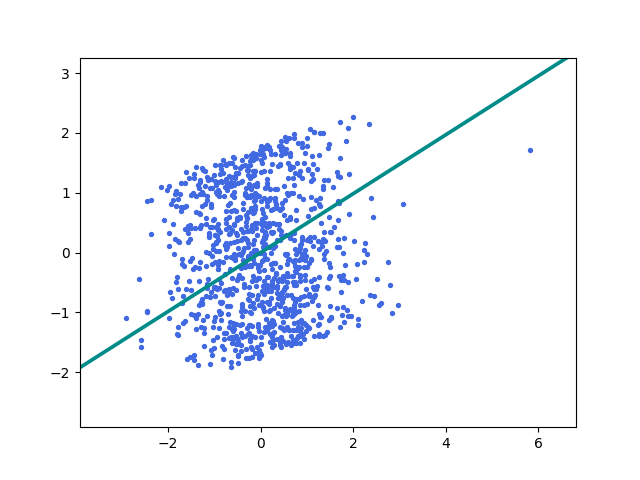
\includegraphics[clip, width=\linewidth]{../figures/assignment2_result_exp_n1000_scatter.png}
            \subcaption{散布図}
            \label{fig:exp_n1000_scatter}
        \end{figure}
    \end{minipage}
    \begin{minipage}{0.45\linewidth}
        \begin{figure}[H]
            \centering
            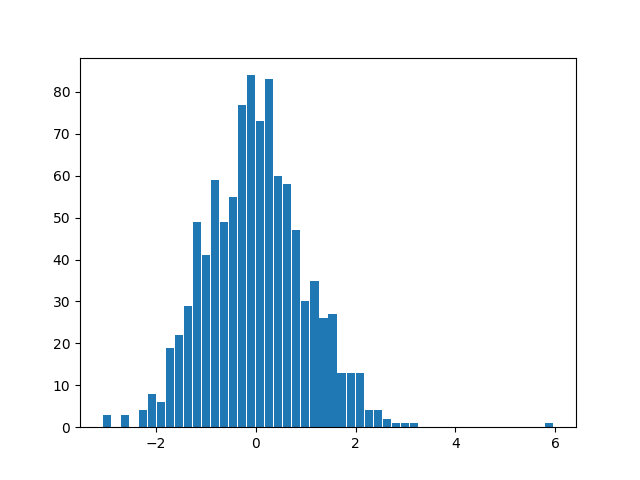
\includegraphics[clip, width=\linewidth]{../figures/assignment2_result_exp_n1000_hist.png}
            \subcaption{ヒストグラム}
            \label{fig:exp_n1000_hist}
        \end{figure}
    \end{minipage}
    \caption{非ガウス性尺度\(G(s) = -\exp(-s^2/2)\),標本数1,000のときの散布図と射影方向,及びヒストグラム}
    \label{fig:exp_n1000}
\end{figure}

\begin{figure}
	\centering
    \begin{minipage}{0.45\linewidth}
        \begin{figure}[H]
        	   \centering
            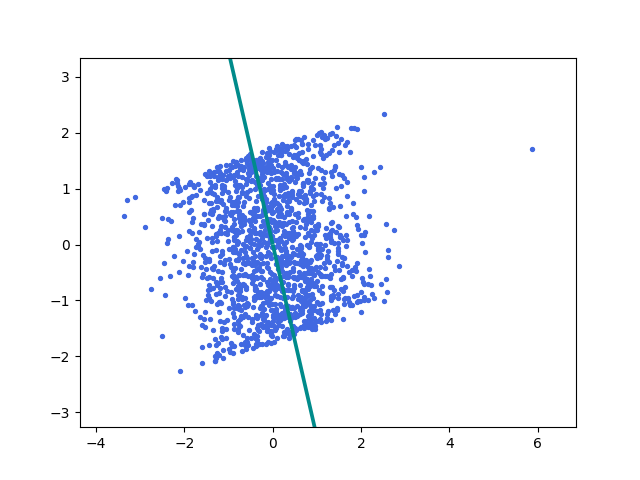
\includegraphics[clip, width=\linewidth]{../figures/assignment2_result_exp_n1500_scatter.png}
            \subcaption{散布図}
            \label{fig:exp_n1500_scatter}
        \end{figure}
    \end{minipage}
    \begin{minipage}{0.45\linewidth}
        \begin{figure}[H]
            \centering
            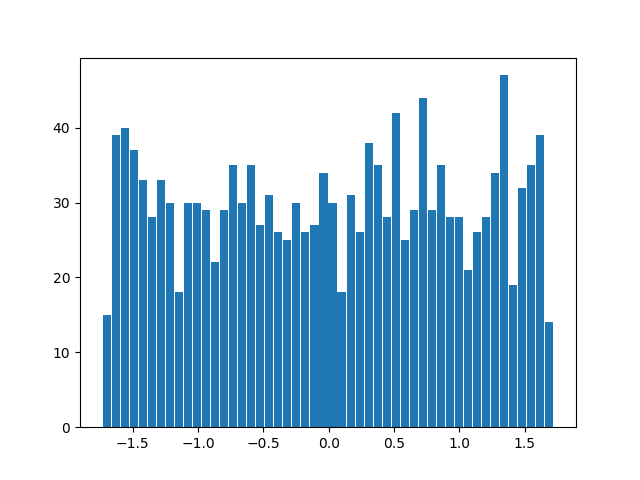
\includegraphics[clip, width=\linewidth]{../figures/assignment2_result_exp_n1500_hist.png}
            \subcaption{ヒストグラム}
            \label{fig:exp_n1500_hist}
        \end{figure}
    \end{minipage}
    \caption{非ガウス性尺度\(G(s) = -\exp(-s^2/2)\),標本数1,500のときの散布図と射影方向,及びヒストグラム}
    \label{fig:exp_n1500}
\end{figure}

\begin{figure}
	\centering
    \begin{minipage}{0.45\linewidth}
        \begin{figure}[H]
        	   \centering
            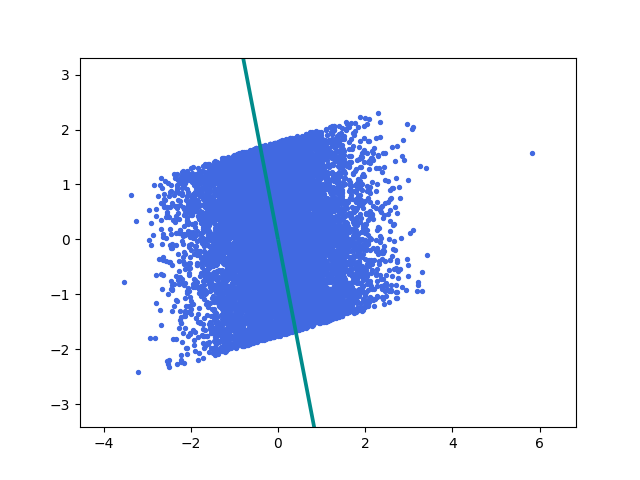
\includegraphics[clip, width=\linewidth]{../figures/assignment2_result_exp_n10000_scatter.png}
            \subcaption{散布図}
            \label{fig:exp_n10000_scatter}
        \end{figure}
    \end{minipage}
    \begin{minipage}{0.45\linewidth}
        \begin{figure}[H]
            \centering
            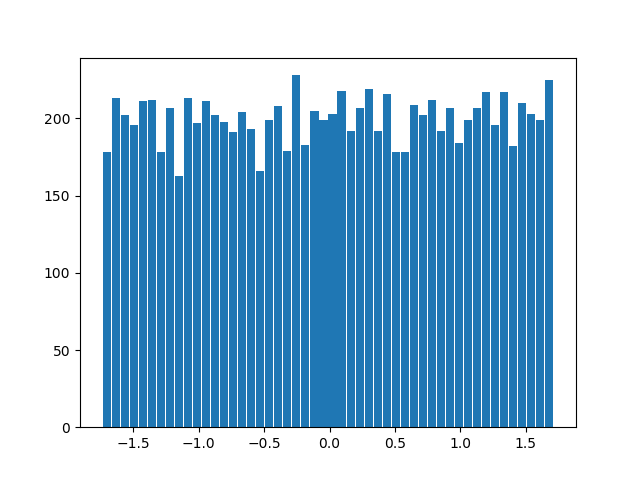
\includegraphics[clip, width=\linewidth]{../figures/assignment2_result_exp_n10000_hist.png}
            \subcaption{ヒストグラム}
            \label{fig:exp_n10000_hist}
        \end{figure}
    \end{minipage}
    \caption{非ガウス性尺度\(G(s) = -\exp(-s^2/2)\),標本数10,000のときの散布図と射影方向,及びヒストグラム}
    \label{fig:exp_n10000}
\end{figure}


\end{document}
